\documentclass[11pt,a4paper]{article}
\usepackage[margin=2.3cm]{geometry}
\usepackage[T1]{fontenc}
\usepackage[utf8]{inputenc}
\usepackage{times}
\usepackage{microtype}
\usepackage{amsmath,amssymb}
\usepackage{booktabs}
\usepackage{array}
\usepackage{enumitem}
\usepackage{graphicx}
\usepackage[hidelinks]{hyperref}
\usepackage{xcolor}
\usepackage{url}
\urlstyle{tt}
\def\UrlBreaks{\do\/\do\_\do\-\do\.}
\usepackage{caption}
\captionsetup{font=small,labelfont=bf}
\setlist{nosep}
\graphicspath{{figures/}}
\newcommand{\pp}{\,\mathrm{pp}}
\newcommand{\code}[1]{\texttt{\small #1}}
\newcommand{\cpath}[1]{{\small\path{#1}}}
\newcommand{\pending}[1]{\begin{center}\fbox{\parbox{0.92\linewidth}{\small\textbf{Pending.} #1}}\end{center}}

\title{HeROsim: graph-aware task placement on a heterogeneous serverless edge\\
\large What the simulator computes, how the labels are made, what the model is, how it is
evaluated, and where the answer stands}
\author{Nikola Luki\'c}
\date{20 September 2026}

\begin{document}
\maketitle

\section{Summary}

\paragraph{The question.} A serverless platform on a cluster of heterogeneous edge devices receives
inference requests from client devices and must place each on a replica (a compute platform on a
machine). Does a graph neural network (GNN) that sees a batch of arriving tasks and the cluster
\emph{as a graph} place them better than (a) the industry-standard reactive scheduler (Knative:
each task to the shortest reachable queue) and (b) a pointwise learned scorer that evaluates one
(task, candidate) pair at a time? The pointwise model is a \emph{control}: if it matches the GNN,
the graph is not what the GNN is using.

\paragraph{The environment in three sentences.} Five measured device platforms (Raspberry~Pi~4
CPU, Nvidia Xavier CPU / GPU / DLA, Xilinx Artix-7 FPGA) with a $7\times$ spread in execution time
and a $60\times$ spread in cold-start time; seeded random client--server topologies over a
store-and-forward backbone; and a workload of real production arrivals in which \textbf{tasks
arrive in peer groups of ten and exchange data with two partners each}, so the cost of a task
depends on \emph{where its partners were placed}. That last ingredient is deliberate: three earlier
lines of work (\S\ref{sec:history}) proved by measurement that in a simulator where every cost is
indexed by a \emph{machine}, the optimal placement is pointwise-separable and a graph model has
nothing to reason about.

\paragraph{How it is measured.} Training labels come from \emph{brute force}: every feasible joint
placement of a task batch is simulated to completion and the cheapest one is the label
(\S\ref{sec:cosim}). Evaluation is a \emph{live gate}: a 50{,}000-event window of the trace
replayed on a cell, learned scheduler against Knative, with bars registered before the data exist
(\S\ref{sec:eval}). The replication unit is an \emph{environment} = (topology, arrival window),
sixteen per rung, because the simulator is deterministic and more tasks buy nothing.

\paragraph{Where the answer stands.}
\begin{itemize}
  \item \textbf{No learned arm beats Knative at any operating point where Knative is healthy.}
  At 6 servers / 40 clients on 16 environments the best arm, \code{gnnedge0}, is $+6.7\,\%$
  \emph{slower} (0/14 checkpoints); at 80 clients $+14.4\,\%$ (0/16); at 80 servers $-1.6\,\%$
  ($p=0.002$), real and far inside the 5\,\% bar (\S\ref{sec:headline}, \S\ref{sec:scale}).
  \item \textbf{The $-20.8\,\%$ headline of 2026-09-18 was an artefact}: an unpaired ratio of
  medians over four cells, two of them saturated. Paired per cell the arm loses three of the
  four (\S\ref{sec:headline}). The record, the reader and the standing answer were corrected on
  2026-09-20.
  \item \textbf{The graph arm is the better learner} (it beats its message-passing-off twin
  $-6.8\,\%$ on 14/14 checkpoints), \textbf{but batching relocates waiting rather than removing
  it}: the 7.1\,s a task waits to assemble its peer group comes back as shorter queues and
  shorter partner-waits, and shortening the window to 2\,s moves the time back without changing
  the total (\S\ref{sec:window}). The arm's genuine gain is 1.05\,s of peer exchange per task
  from co-location; its genuine cost is the concentration that produces.
\end{itemize}
Two caveats travel with every number: the arrival window every earlier gate used (w0) is the
burstiest of the four the trace offers, and the peer payloads are a synthetic augmentation of a
real trace (\S\ref{sec:peer}).

\section{The environment}
\label{sec:env}

\subsection{Heterogeneous hardware}

The simulator (SimPy, discrete-event, single-threaded) models machines with a hardware class, a set
of \emph{platforms} (one task at a time each, FIFO queue), a memory budget, local flash storage
with capacity-bounded image eviction, and a network map. Three hardware classes are used in the
gate cells, assigned round-robin to machines: a Raspberry~Pi~4 (four CPU platforms, 8\,GB), a
Xavier system-on-module (eight CPU platforms, one GPU, one DLA) and a PYNQ board (one FPGA). Each
task type carries a \emph{measured} table per platform type (Table~\ref{tab:devices}), not a
scaling factor; the platform that runs a task fastest is often the slowest to start.

\begin{table}[h]
\centering\small
\begin{tabular}{llrrrr}
\toprule
task type & platform & execution (s) & cold start (s) & memory (GB) & image (GB) \\
\midrule
dnn1 & rpiCpu & 0.0029 & 0.33 & 0.066 & 3.06 \\
dnn1 & xavierCpu & 0.0010 & 0.071 & 0.069 & 2.99 \\
dnn1 & xavierGpu & 0.0208 & 6.17 & 0.900 & 2.99 \\
dnn1 & pynqFpga & 0.0006 & 0.98 & 0.000 & 0.004 \\
dnn2 & rpiCpu & 0.1684 & 0.636 & 0.069 & 3.06 \\
dnn2 & xavierCpu & 0.0239 & 0.096 & 0.069 & 2.99 \\
dnn2 & xavierGpu & 0.0362 & 6.14 & 0.900 & 2.99 \\
\bottomrule
\end{tabular}
\caption{The measured per-platform tables for the two inference types in the gate workload
(\code{data/nofs-ids/task-types.json}). A 3\,GB image pull at 100\,MB/s is 31.3\,s and serialises
on the machine's disk.}
\label{tab:devices}
\end{table}

\subsection{Topology}

Topologies are generated deterministically from a seed (\cpath{src/generate_infrastructure.py}):
client machines and server machines, client--server links drawn independently with probability
0.6 with per-device-pair latency ranges (30--150\,ms), a repair step so that every client reaches
at least two replica-hosting servers, and a backbone of 12 core routers (1\,Gbps, 4\,ms per core
link, 20\,ms access links) through which every logical link is routed. Transmission over the
backbone is store-and-forward: each hop is a capacity-one pipe held for $\text{bytes}/\text{bandwidth}$,
so only \emph{shared} core segments couple two tasks' transfers (\cpath{src/placement/network_fabric.py}).
Figure~\ref{fig:topo} shows the cell on which the headline was first read.

\begin{figure}[h]
\centering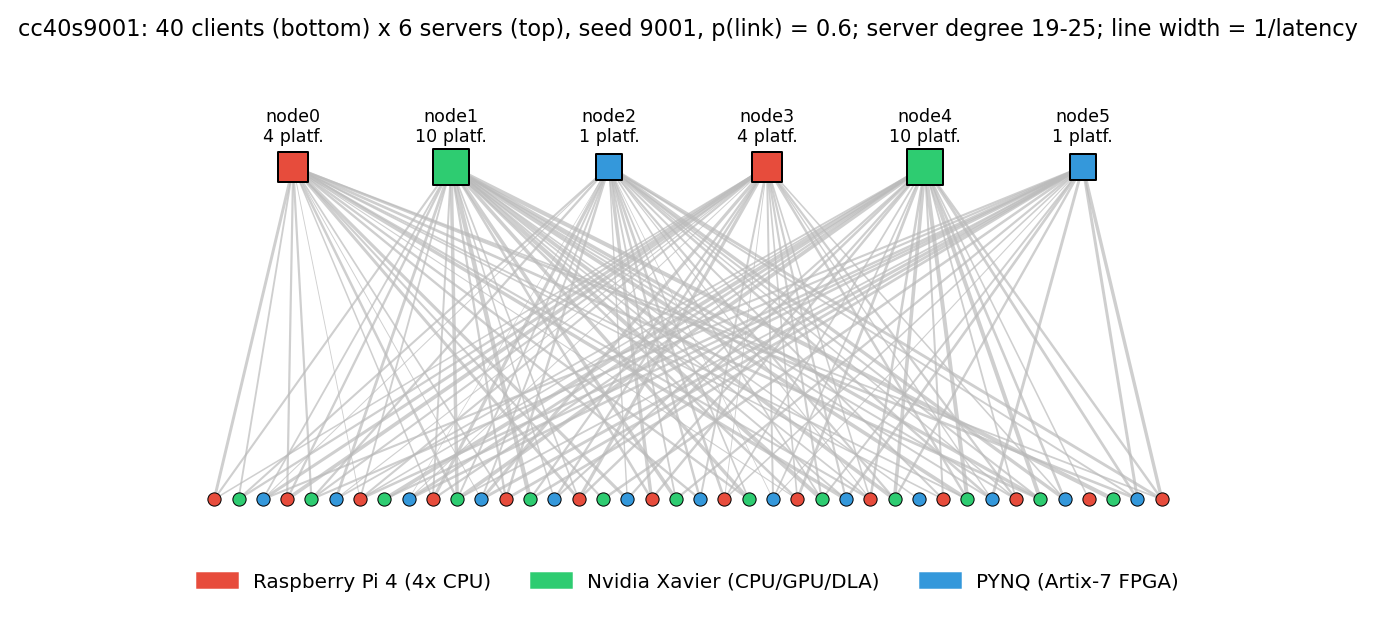
\includegraphics[width=\linewidth]{fig1_topology}
\caption{Cell \code{cc40s9001}: 40 clients, 6 servers, topology seed 9001. Server squares are sized
by platform count; servers host one replica per task type. Adding clients keeps each task's
candidate set inside the training corpus's support (3--5 candidates per task), adding servers
does not (48 at 80 servers).}
\label{fig:topo}
\end{figure}

\subsection{How a response time is composed}

A task's response time runs from dispatch to completion. In order, the platform's processing
loop charges: (1) \textbf{scheduler wait} --- for the learned arms, the time spent assembling the
task's peer group before a decision (\S\ref{sec:peer}); (2) \textbf{FIFO queueing} behind the tasks
already on the chosen platform; (3) propagation latency from the source machine; (4) ingress and
per-link transmission waits over the backbone; (5) the \textbf{image pull} if the machine's disk
does not hold the image, serialised with other pulls on that disk; (6) the platform-specific
\textbf{cold start} unless the previous task on the platform had the same type; (7) input read plus
the \textbf{peer exchange} with every partner placed on another machine; (8) execution, a table
lookup; (9) output write. Nothing dilates: a co-resident never changes how long a task's own
computation takes; every interaction is a \emph{wait before work starts}. Given infrastructure,
workload and placements the loop contains no random draws, so an episode is deterministic --- a
fact that shapes the evaluation design (\S\ref{sec:eval}). Figure~\ref{fig:comp} shows where the
time goes for the three schedulers that matter.

\begin{figure}[h]
\centering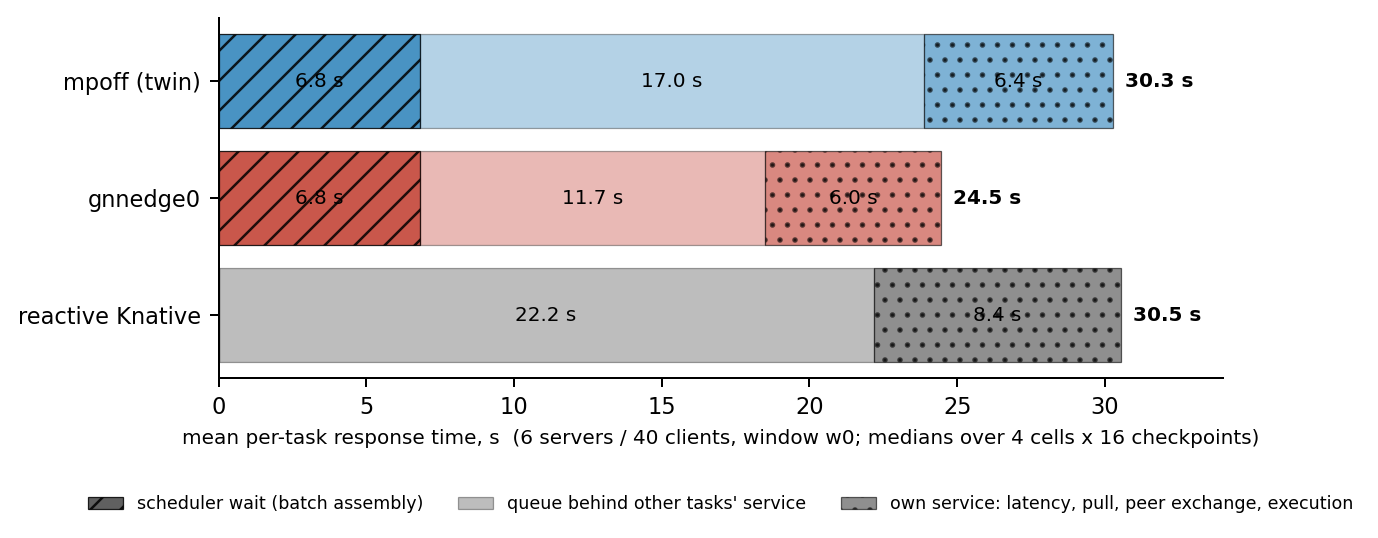
\includegraphics[width=\linewidth]{fig2_composition}
\caption{Per-task response time decomposed, 6 servers / 40 clients, window w0. The learned arms
pay $\approx 6.8$\,s of scheduler wait that Knative never pays, and win back more than that in
queue; the pointwise twin (\code{mpoff}) pays the same wait and does not win it back.}
\label{fig:comp}
\end{figure}

Warmth follows the \code{node\_disk\_v2} physics (ADR~0001): a warm sandbox skips the cold start,
and only a node-local disk hit skips the pull, so a warm sandbox never masks an evicted image. The
earlier \code{platform\_reuse\_v1} rule is retained only so that old corpora stay bit-reproducible.

\subsection{Why tasks communicate: the peer exchange}
\label{sec:peer}

\paragraph{The argument.} Sections \ref{sec:history} and the September~9 report establish, by
measurement, that if every contention term is indexed by a machine (queue, disk, memory, ingress
pipe), by the task's own platform (warmth) or by a link on its own route, then co-residents are
exchangeable within a task type, every symmetric function of a multiset is a function of its
counts, and a pointwise scorer that is told the per-machine counts can express the exact cost. A
graph model has no additional fact to work with, and it measurably ties. The one kind of cost that
escapes this argument is one indexed by a \emph{pair of task instances} decided jointly: the price
of placing $i$ and $j$ apart cannot be written as a function of any machine's counts.

\paragraph{The mechanism.} A workload carries a table of peer pairs $(i, j, \text{bytes})$. At
task $i$'s input stage, for every partner $j$
(\cpath{src/placement/infrastructure.py}, \cpath{_peer_exchange_time}):
\[
c_{ij} \;=\; \begin{cases} 0 & \text{if } i \text{ and } j \text{ run on the same machine,}\\[2pt]
\text{hops}(m_i, m_j)\cdot \dfrac{\text{bytes}_{ij}}{\min_{\ell \in \text{route}} \text{bw}_\ell} + \text{latency}(m_i, m_j) & \text{otherwise,}\end{cases}
\]
charged into the task's service time (so it also inflates the queue of everyone behind it), plus a
\emph{rendezvous wait} if $j$ has not been placed yet. Dividing by the receiving machine's own
bandwidth, an earlier form, made the term separable again --- a $100{,}000\times$ payload scaling
probe left additive-argmin regret at exactly 0.000\,\%; the hop count is what gives distance
magnitude. Every legacy corpus is bit-identical with the mechanism off.

\paragraph{The workload, stated honestly.} The arrival trace is the project's own production
capture (\cpath{workload-150-150.json}: 450{,}729 single-task events at 150 requests/s over 20
clients, two DNN types), \emph{not} a public dataset. The peer pairs are a \emph{synthetic
augmentation} of it:\footnote{\cpath{scripts_cosim/make_peer_affinity_production_workload.py}, whose usage line builds exactly the gate file.}
consecutive arrivals are grouped in tens, every task draws two distinct partners inside its
group, and each pair's payload is $200\,\text{MB}\times 10^{U(-1,1)}$; the draw is seeded and the
provenance (seed, source hash, pair count) is written into the file. The transfer physics is
checked; the payload distribution is an assumption, and the report says so wherever a number
depends on it. Figure~\ref{fig:peer} shows the resulting group structure and the fact that decides
the scheduler's cost: a group's ten members arrive over a median 13.8\,s.

\begin{figure}[h]
\centering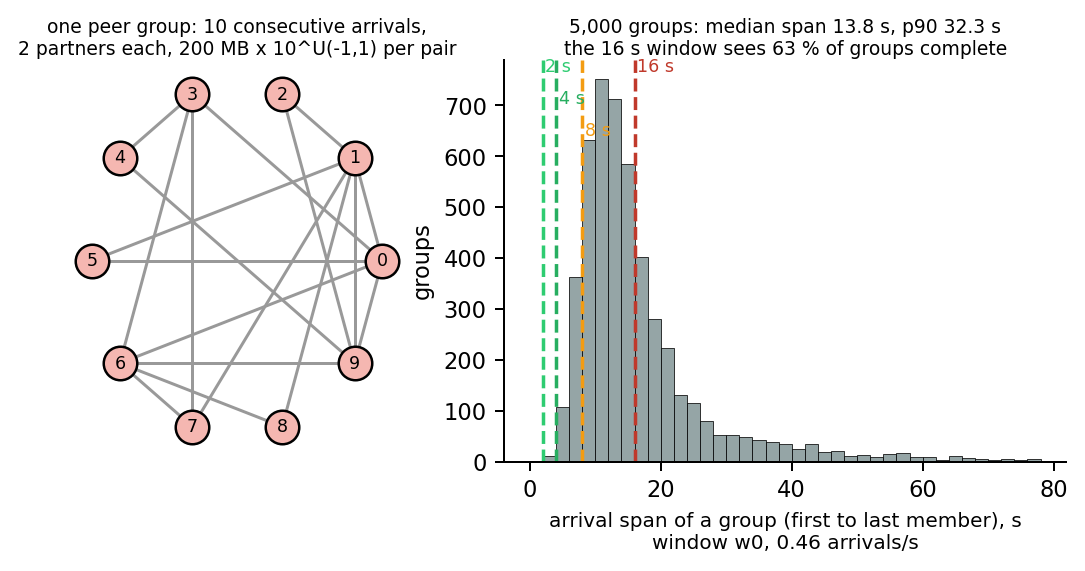
\includegraphics[width=\linewidth]{fig3_peer_groups}
\caption{Left: one peer group. Right: the arrival span of the 5{,}000 groups in the 50{,}000-event
gate window at 0.46 arrivals/s, against the four batch windows studied in \S\ref{sec:window}. A
learned arm that waits for the whole group pays about half the span per task.}
\label{fig:peer}
\end{figure}

\subsection{Is it checked?}

\begin{itemize}
  \item \textbf{Determinism.} Seeded topology, replicas, workload draw and training. Re-running a
  (cell, workload, policy) triple is bit-identical: the reactive run on \code{cc40s9001} made for
  tonight's screen equals the one made two days ago to the last digit of \code{total\_rtt}. A test
  runs every trainer twice at a fixed seed and requires identical weights.
  \item \textbf{Fail-loud contracts.} Every checkpoint carries a sidecar naming its feature
  contract, physics, corpus split hash and every architecture flag invisible in the weights;
  serving refuses a mismatch instead of adopting a default. Every gate script pins, per arm, the
  flags that separate it from its twin.
  \item \textbf{Registration.} Every lineage commits its bars, reader and tests \emph{before} its
  data exist, records its expectation, and closes only on a live gate (rule 6 of the record).
  \item \textbf{What the discipline caught.} A batch-timeout precedence bug (a 4{,}000$\times$
  window served as 20\,ms); a queue feature out of its training range by $300\times$; an unseeded
  trainer that made every early MLP checkpoint an unreproducible draw; a cluster environment leak
  that ran three sessions of gates on an undeclared interpreter; and, tonight, 15 topology cells
  that hang in a known starved-client spin, cancelled and excluded by rule.
\end{itemize}

\section{Brute-force labelling by co-simulation}
\label{sec:cosim}

Supervised training needs, for a cluster state and a batch of tasks, the joint placement that
actually minimises the batch's cost in the simulator. The pipeline (Figure~\ref{fig:cosim};
\code{src/executecosimulation.py}) produces it by exhaustive enumeration.

\begin{figure}[h]
\centering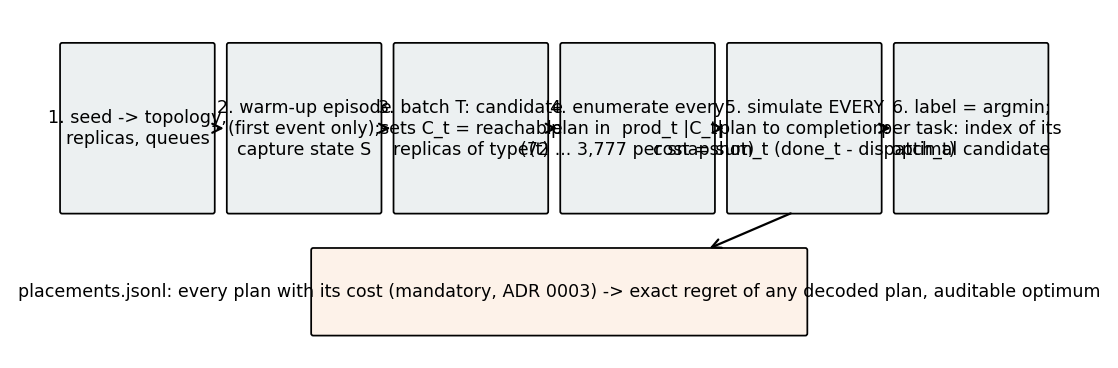
\includegraphics[width=\linewidth]{fig4_cosim}
\caption{One dataset (snapshot) of the co-simulation corpus.}
\label{fig:cosim}
\end{figure}

Let $S$ be the system state after a warm-up episode that runs only the first workload event, and
let $T$ be the batch. For each $t\in T$ the candidate set $C_t$ is every (machine, platform) that
holds a replica of $t$'s type and is reachable from $t$'s client. A plan is $\pi\in\prod_t C_t$
(optionally restricted to distinct replicas). Every plan is simulated to completion with the
placement forced, and its cost is the episode's total response time,
\[
J(\pi) \;=\; \sum_{t\in T}\big(\text{done}_t(\pi) - \text{dispatch}_t\big),
\qquad \pi^\star = \arg\min_\pi J(\pi),
\]
warm-up tasks excluded. The label of task $t$ is the index of $\pi^\star_t$ within $C_t$. The full
sweep $\{(\pi, J(\pi))\}$ is written to \code{placements.jsonl} and is \emph{mandatory} (ADR~0003):
it makes the optimum auditable and the \emph{regret} of any decoded plan, $J(\hat\pi)-J(\pi^\star)$,
an exact lookup. Sweeps hold 72 to several thousand plans per snapshot; datasets whose product
exceeds a threshold are skipped with the reason recorded, so a void corpus is never misread. The
corpora used here hold 1{,}670 snapshots (and a 516-snapshot subset for corpus-matched controls),
split 1{,}524 / 96 / 34 by a committed artefact whose hash every checkpoint carries: \emph{a
corpus is its split, not its directory}.

\paragraph{Prefix-conditioned labels (\code{partial\_state\_v3}).} Live decoding commits tasks one
at a time, so the corpus is written the same way: for task $k$ the feature row of every candidate
carries a 22-dimensional \emph{prefix block} describing what tasks $1..k-1$ have already committed
on that candidate's machine (type occupancy, committed and remaining demand against capacity, rank
of the candidate among its type as a size-free fraction). The earlier 38-dimensional block encoded
ranks as a one-hot over at most five machines, which pinned every checkpoint to 6-server cells; the
size-free block is what lets a 6-server checkpoint be served on 80 servers at all.

\section{The model and its training}
\label{sec:model}

\begin{figure}[h]
\centering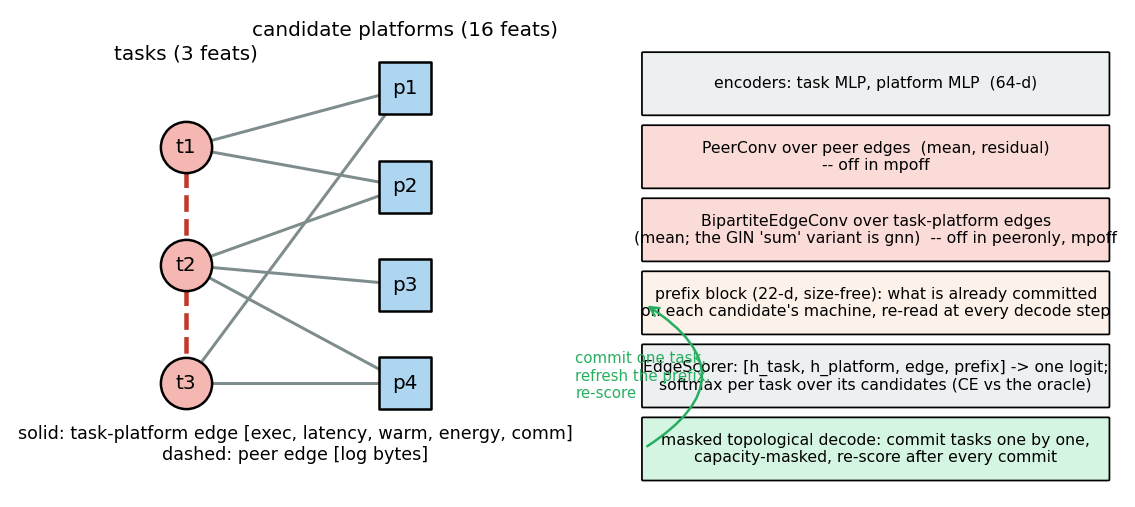
\includegraphics[width=\linewidth]{fig5_model}
\caption{The bipartite graph and the stages of the scoring network. The five arms differ only in
which shaded stages are active.}
\label{fig:model}
\end{figure}

Each snapshot is one graph (Figure~\ref{fig:model}): task nodes (type one-hot, source) and
candidate-platform nodes (16 physics features: platform type, queue depth, warmth, remaining work,
pull backlog, \ldots), task--platform edges carrying [execution time, latency, is-warm, energy,
communication time], and task--task \emph{peer edges} carrying $\log(1+\text{bytes}/10^6)$. Two
message-passing stages follow the encoders:
\begin{itemize}
  \item \textbf{PeerConv} over peer edges: $h_i \leftarrow h_i + \mathrm{MLP}\big([h_i;
  \mathrm{mean}_{j\sim i}\,\mathrm{MLP}([h_j; e_{ij}])]\big)$ --- residual, mean aggregation.
  \item \textbf{BipartiteEdgeConv} over task--platform edges, same message form, \textbf{mean}
  aggregation over a task's candidates. The original arm (\code{gnn}) used a GIN with \emph{sum}
  aggregation; a sum over a candidate set that is 3.6 wide at 6 servers and 47.9 at 80 makes the
  layer a function of deployment size, and that alone cost $+13\,\%$ at 80 servers and nothing at
  6 (\cpath{bipartite_aggr_v1}: \cpath{SUM-COSTS-ONLY-WHERE-CANDIDATES-ARE-MANY}).
\end{itemize}
An \textbf{EdgeScorer} maps $[h_t; h_p; e_{tp}; \text{prefix}_{tp}]$ to one logit per
(task, candidate); logits are grouped per task. Decoding is \emph{masked topological}: tasks are
committed one by one, candidates masked by machine capacity, the prefix block refreshed and every
remaining task re-scored after each commit; there is no unmasked fallback and a failed decode is an
error. The same closure computes the prefix at training and at serving time, so the two cannot
drift.

\begin{table}[h]
\centering\small
\begin{tabular}{lccc p{5.6cm}}
\toprule
arm & PeerConv & bipartite stage & aggregation & role \\
\midrule
\code{gnn} & on & GIN & sum & the original bipartite arm \\
\code{gnnedge} & on & EdgeConv & mean & the repair, edge attributes on \\
\textbf{\code{gnnedge0}} & on & EdgeConv & mean & \textbf{the headline arm}; attributes zeroed, matched \code{gnnedge} ($+0.44\,\%$, 8/16) \\
\code{peeronly} & on & none & --- & peer edges alone \\
\code{mpoff} & \textbf{off} & none & --- & the pointwise twin: identical weights layout, no message passing \\
\bottomrule
\end{tabular}
\caption{The arms. All trained on the same 1{,}670-snapshot corpus and split, 16 seeds each.}
\end{table}

\paragraph{Training} (\cpath{run_experiment.py} over a YAML per arm; trainer
\cpath{src/notebooks/train_near_rtt.py}). Per-task cross-entropy over the task's candidates
against the brute-force optimum; AdamW at $2\times10^{-3}$; up to 300 epochs with patience 60 and a
100-epoch floor; the checkpoint is chosen by \emph{validation decode regret} (exact, from the
sweeps), never the last epoch --- selected-vs-last is worth $+13$--$16\,\%$ live. Sixteen seeds per
arm; every run logs to Weights~\&~Biases; every checkpoint is saved with its contract sidecar.
Arms differ by exactly one flag in their YAML, so at a fixed seed \code{gnnedge0} and its twin start
from bit-identical weights and differ in one operation.

\section{Evaluation design}
\label{sec:eval}

\subsection{The live gate and why 50{,}000 tasks}

A live gate replays a window of the trace on a cell: the policy under test receives arrivals in
simulated time, scales replicas, places tasks, and the metric is the mean per-task response time
(\code{averageElapsedTime}). One run is 50{,}000 events, rescaled to 0.46 arrivals/s (30.2 hours
of simulated time, about three minutes of wall clock). Three facts fix the design:
\begin{enumerate}
  \item \textbf{Task count is not a lever.} Because an episode is deterministic, one (environment,
  checkpoint) run carries \emph{zero} sampling noise. All the variance in a checkpoint's score is
  interaction with the environment, and the standard deviation of the checkpoint statistic scales
  as exactly $1/\sqrt{n_{\text{environments}}}$ (measured: 36.4 $\to$ 18.1\,pp from one cell to
  four). A longer trace only averages more load regimes into one number; it tightens nothing.
  \item \textbf{The baseline must be healthy.} Knative's capacity does not grow with the cluster:
  80 servers are unsaturated only at the \emph{same} 0.46 arrivals/s that 6 servers run at
  (Figure~\ref{fig:ladder}). Every earlier ``$-30$ to $-47\,\%$ at 80 servers'' was read against a
  baseline pushed $13\times$ past a ceiling that never moved. A cell enters a study only if
  reactive's queue share (queue / response time) is $\le 0.80$; a cell that hangs is
  \emph{unreadable}, and unknown is not a pass.
  \item \textbf{The window is not ``the workload''.} Every gate before this week used the first
  50{,}000 events of the trace. That window is $1.6\times$ slower natively (the ramp-in) and, once
  rate-matched, the burstiest of the four the trace offers (Figure~\ref{fig:windows}). Each window
  therefore gets its own rescale factor so that all four deliver 0.4604 arrivals/s and the window
  axis is arrival \emph{pattern}, not load.
\end{enumerate}

\begin{figure}[h]
\centering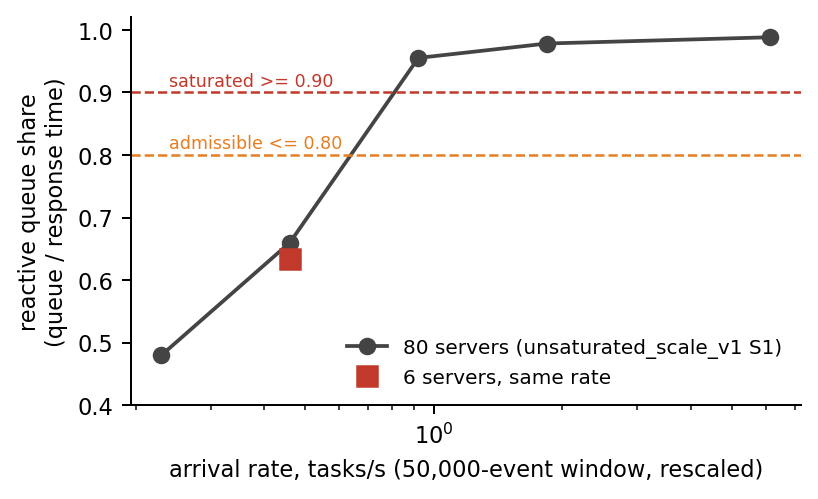
\includegraphics[width=0.62\linewidth]{fig7_load_ladder}
\caption{Reactive Knative's queue share against arrival rate (\code{unsaturated\_scale\_v1}).
The 80-server cluster is healthy only at the rate 6 servers run at.}
\label{fig:ladder}
\end{figure}

\begin{figure}[h]
\centering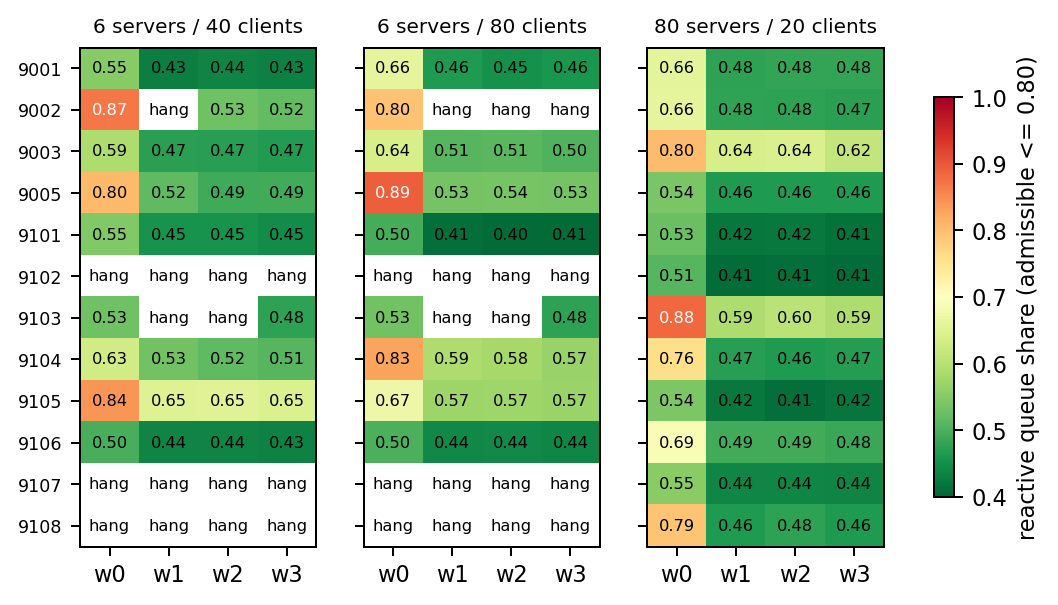
\includegraphics[width=\linewidth]{fig8_windows}
\caption{Reactive queue share per candidate topology and arrival window on the three rungs
studied (the saturation screens). Every saturated cell is a w0 cell; 15 cells per 6-server rung
hang in the starved-client spin (a recorded simulator defect) and are inadmissible. The four
lowest-numbered topologies admissible on all four windows form each rung's study.}
\label{fig:windows}
\end{figure}

\subsection{The statistic and the bars}

An \emph{environment} is a (topology, window) pair; a study is $4\times4=16$ of them, fully
crossed. The \textbf{unit is the checkpoint} (16 per arm). For checkpoint $s$ and environment
$e$ let $r_{s,e} = 100\,(\text{elapsed}_{s,e}/\text{elapsed}^{\text{ref}}_{e} - 1)$, the relative
difference against the reference \emph{on the same environment}; the checkpoint statistic is
$\mathrm{median}_e\, r_{s,e}$. Arm-vs-arm contrasts pair raw elapsed times on both environment and
checkpoint. Every read is a two-sided Wilcoxon signed-rank test of the 16 statistics against zero
and fires only if $|\text{median}| \ge 5\,\%$ \emph{and} $p<0.05$; a significant $1.6\,\%$ is
reported as real and \emph{not separated}. A design-power bar (worst-arm sd $\le 10\,$pp) is read
first, so an under-powered negative is never called a tie. Topologies are selected by the lowest
seed ids admissible on every window --- a rule no arm can steer. Baselines on every environment:
\code{knative\_network} (the reference), \code{knative\_network\_ect} (expected completion time),
\code{random\_network}. (\code{knative\_network\_batch} was measured at 0.002\,s of batch wait and
is a second reactive variant, not a batching control.)

\section{Results}
\label{sec:results}

\subsection{What came before, in one section}
\label{sec:history}

The programme's first month (record 2026-08-17 to 09-09, September~9 report) ran three routes to a
positive answer and closed all three by measurement. Learned schedulers beat Knative by a wide
margin on the original corpus ($-44.8\,\%$ on a held-out fabric), but every advantage of the GNN
over a pointwise MLP vanished under a matched control: a pointwise model trained on the same
corpus ties the GNN on latency; the reliability edge was 87\,\% a corpus effect and not
established once matched ($p=0.11$, $n=16$); message passing was a null ingredient on every graph
tried ($p=0.37$, $p=0.25$). The structural reason (count-shaped costs, \S\ref{sec:peer}) was
corroborated by a one-integer control and by an additive fit with $R^2=1.00000$ on plans that place
every task on a distinct machine. Two alternatives to the supervised target were measured
negative: multi-step horizon labels are deterministic chaos, and closed-loop policy gradient does
not improve the supervised checkpoint ($n=120$, $p=0.93$). The peer-exchange environment
(\code{peer\_affinity\_v1}) followed from that argument, and its first positive was offline: message
passing beats its twin by $+5.14\,$pp ($p=0.001$, 13/16) at 482 snapshots, reproduced at 1{,}654.
Offline edges then had to be taken live, which is where the rest of this section lives.

\subsection{The headline at power: 6 servers, 40 and 80 clients}
\label{sec:headline}

Between 2026-09-16 and 09-18 four lineages (\cpath{peer_only_v1}, \cpath{bipartite_edge_v1},
\cpath{bipartite_aggr_v1}, \cpath{best_arm_v1}) reported, on four cells of window w0 with 16
checkpoints each, that \code{gnnedge0} beats Knative by $-20.8\,\%$ at 40 clients and $-13.5\,\%$
at 80. \cpath{unsaturated_edge_v1} (registered 2026-09-19, commit \code{96f0b69}; closed
2026-09-20) re-measured the headline on 16 environments per rung with the same checkpoints and
bars, and found two things.

\paragraph{The headline was an unpaired statistic.} The earlier reader collapsed each
checkpoint to the \emph{median of the arm over the four cells} and divided by the \emph{median of
Knative over the four cells}. Those two medians come from different cells; Knative's time on the
four ranged from 18 to 64\,s. Read \emph{paired}, cell by cell, the same data give:

\begin{table}[h]
\centering\small
\begin{tabular}{lrrrrrr}
\toprule
40 clients, w0 & 9001 (share 0.55) & 9002 (0.87) & 9003 (0.59) & 9005 (0.80) & old statistic & paired \\
\midrule
\code{gnnedge0} & $+4.6$ & $+75.8$ & $+9.7$ & $-36.8$ & $-20.3\,\%$ & $\mathbf{+7.0\,\%}$ \\
\code{peeronly} & $+6.9$ & $+60.4$ & $+11.7$ & $-33.4$ & $-14.9\,\%$ & $\mathbf{+9.4\,\%}$ \\
\code{mpoff} (twin) & $+13.2$ & $+57.2$ & $+32.0$ & $+13.8$ & $+18.5\,\%$ & $+22.0\,\%$ \\
\bottomrule
\end{tabular}
\caption{The four original headline cells, per cell (\% vs Knative, medians over 16 checkpoints).
The two cells Knative was slow on are the two that fail the saturation bar; the arm wins only on
one of them and loses the other catastrophically.}
\end{table}

\paragraph{On 16 admissible environments, every learned arm loses to Knative.}
Figure~\ref{fig:headline} and Table~\ref{tab:e1}. The design delivered its power (worst-arm sd
1.2\,pp at 40 clients, 2.9 at 80, against the 10\,pp bar); every arm keeps its sign on all four
windows; \code{gnnedge0} and \code{gnn} are \emph{unreadable by the letter} at 40 clients because 2
and 4 of their 256 arms hang deterministically in the starved-client spin (the reader refuses a
ragged design), and their reads on the complete checkpoints are reported as \emph{disclosed}.

\begin{table}[h]
\centering\small
\begin{tabular}{llrrl}
\toprule
rung & arm & vs Knative & vs random & verdict \\
\midrule
40 cl. & \code{gnnedge0} & $+6.68\,\%$, 0/14, $p=0.001$ & $-4.47\,\%$, 14/14 & disclosed ($n=14$) \\
40 cl. & \code{peeronly} & $+8.36\,\%$, 0/16, $p=0.0004$ & $-1.42\,\%$ & \code{REACTIVE-FASTER} \\
40 cl. & \code{mpoff} (twin) & $+11.53\,\%$, 0/16, $p=0.0004$ & $+1.72\,\%$ & \code{REACTIVE-FASTER} \\
40 cl. & \code{gnn} (sum) & $+9.24\,\%$, 0/12, $p=0.002$ & $-1.19\,\%$ & disclosed ($n=12$) \\
80 cl. & \code{gnnedge0} & $+14.40\,\%$, 0/16, $p=0.0004$ & $-0.23\,\%$ (tie) & \code{REACTIVE-FASTER} \\
\midrule
40 cl. & \code{gnnedge0} vs \code{mpoff} & \multicolumn{2}{l}{$\mathbf{-6.82\,\%}$, 14/14, $p=0.001$} & \code{GRAPH-FASTER} \\
40 cl. & \code{gnn} vs \code{gnnedge0} & \multicolumn{2}{l}{$+2.12\,\%$, $p=0.01$} & \code{SUM-NOT-SEPARATED} \\
\bottomrule
\end{tabular}
\caption{The registered reads on 16 environments per rung (unit = checkpoint; median over
environments of the paired relative \%). Knative's median response time is 17.9\,s at 40 clients
and 18.3\,s at 80; random placement is $+4.5\,\%$ and $+13.9\,\%$ behind it.}
\label{tab:e1}
\end{table}

\begin{figure}[h]
\centering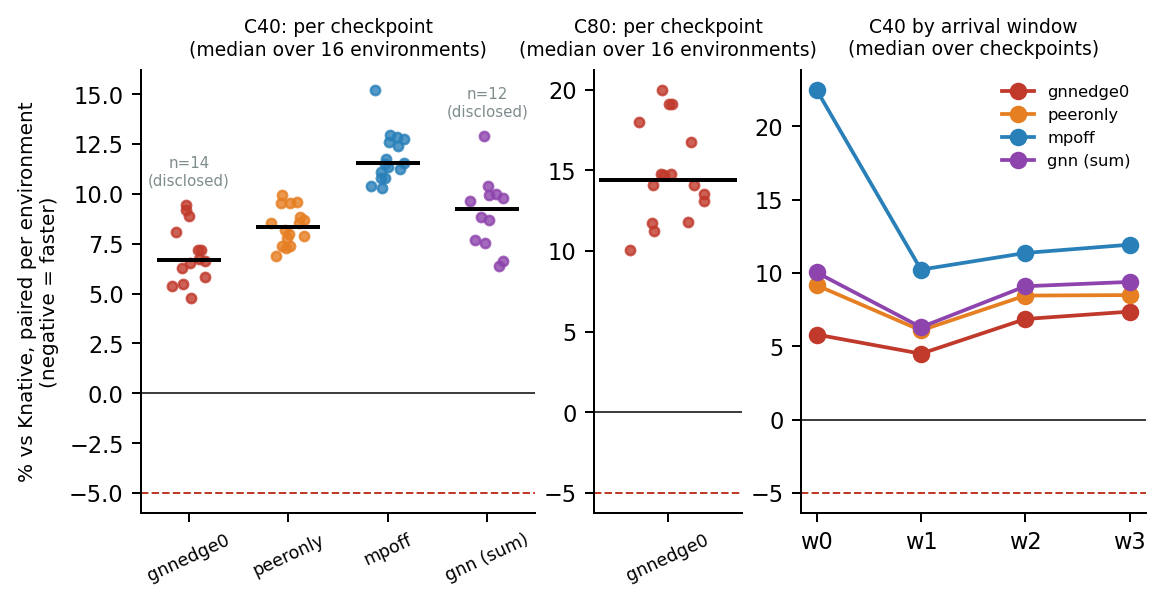
\includegraphics[width=\linewidth]{fig9_headline}
\caption{Left, middle: the 16 checkpoint statistics per arm against Knative at 40 and 80
clients (bar = median; dashed = the $-5\,\%$ bar). Right: the 40-client medians by arrival window.
Nothing is below zero.}
\label{fig:headline}
\end{figure}

\paragraph{What survives, and what it means.} The graph arm is the better \emph{learner}:
it beats its message-passing-off twin on 14 of 14 checkpoints, paired on environment and
checkpoint, and the \emph{sum} penalty is absent at 6 servers exactly as \cpath{bipartite_aggr_v1}
predicted. Where the deficit sits is the subject of \S\ref{sec:window}: the arm pays 7.1\,s of
scheduler wait per task, and the question is whether that wait is a tax on top of a good
placement or the same waiting booked elsewhere.


\subsection{At scale: 80 servers}
\label{sec:scale}

\code{unsaturated\_scale\_v1} found the capacity fact of Figure~\ref{fig:ladder} and, at the one
healthy rung, that no arm beats Knative on four cells; \code{unsaturated\_scale\_v2} re-read the
same five quantities on 16 environments (1{,}328 arms, 0 failures, worst-arm sd 4.48\,pp against
the 10\,pp design bar). Figure~\ref{fig:v1v2} is the finding: \textbf{every direction replicated,
every magnitude collapsed}, because the four v1 cells were all window w0. \code{gnnedge0} is
$-1.62\,\%$ ($p=0.0023$, 13/16), \code{peeronly} $-1.23\,\%$ ($p=0.0013$, 15/16), the GIN-sum arm
loses $+2.31\,\%$, the matched model-class edge is $-2.38\,\%$ ($p=0.0004$) --- all real, all
inside the 5\,\% bar. The batch-assembly wait is 7.12--7.13\,s for every learned arm and 0.000\,s
for Knative, ECT and random: 37\,\% of Knative's 19.1\,s response time, and the arms win back
almost exactly that much queue. \code{random\_network} is $+8.4\,\%$ behind Knative in median with
a bimodal tail to $+782\,\%$.

\begin{figure}[h]
\centering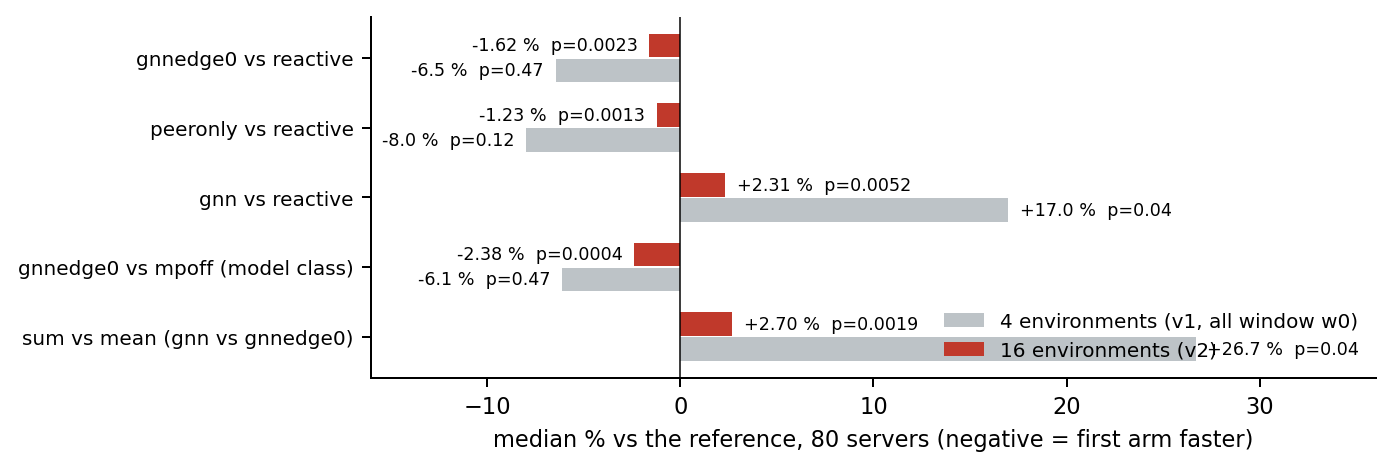
\includegraphics[width=\linewidth]{fig10_v1_vs_v2}
\caption{Quote a direction from a small design and a magnitude only from a large one: the five
registered quantities at 80 servers, four environments (all w0) against sixteen.}
\label{fig:v1v2}
\end{figure}

\subsection{The batch tax and the window}
\label{sec:window}

Every learned arm collects a task's whole peer group before it decides, waiting up to
\code{batch\_timeout} $=16$\,s for members not yet arrived; with group spans of median 13.8\,s
(Figure~\ref{fig:peer}) that is 6.8\,s per task. The window is a policy constant set once and
swept once, at the 20-client rung where every learned arm loses to Knative by $\ge 70\,\%$
whatever the window. \code{batch\_window\_edge\_v1} (registered 2026-09-19, commit \code{f6384eb})
screens 2 / 4 / 8\,s on the lowest-seed study topology (four windows, 16 checkpoints) and confirms
the chosen window on the twelve held-out environments, \code{gnnedge0} and its twin, with a
mechanism read (W6: the wait must actually fall) gating the interpretation.

\paragraph{Result: the window is not the lever.} Table~\ref{tab:bw} and
Figure~\ref{fig:bw}. On the screen topology the scheduler wait falls from 7.15\,s to 1.66\,s as
the window shortens from 16 to 2\,s, and the median against Knative does not move: $+7.70\,\%$
at 16\,s, $+7.87$ (4\,s), $+8.04$ (8\,s), $+8.77$ (2\,s). The registered rule picks the incumbent
(4 and 8\,s are ineligible by the letter because one and two of their arms hang in the
starved-client spin; the disclosed reads on the complete checkpoints agree), so the lineage
closes \code{WINDOW-NOT-THE-LEVER} on its screen and the held-out phase does not run.

\begin{table}[h]
\centering\small
\begin{tabular}{lrrrrr}
\toprule
window & wait / task & median vs Knative & w0 / w1 / w2 / w3 & queue (w1) & rendezvous (w1) \\
\midrule
2\,s & 1.66\,s & $+8.77\,\%$ & $+9.3$ / $+8.9$ / $+8.6$ / $+8.5$ & 8.19\,s & 3.34\,s \\
4\,s & 2.65\,s & $+7.87\,\%$ (n=15) & $+5.7$ / $+8.9$ / $+8.0$ / $+7.7$ & 7.34 & 3.20 \\
8\,s & 4.30\,s & $+8.04\,\%$ (n=14) & $+4.0$ / $+8.7$ / $+7.9$ / $+8.1$ & --- & --- \\
16\,s & 7.15\,s & $\mathbf{+7.70\,\%}$ & $+4.6$ / $+8.5$ / $+7.4$ / $+8.2$ & 4.78 & 1.2 \\
\bottomrule
\end{tabular}
\caption{\code{gnnedge0} on the screen topology (\code{cc40s9001}, four arrival windows, 16
checkpoints) at four batch windows. What the scheduler releases, the platform queue and the
rendezvous wait absorb.}
\label{tab:bw}
\end{table}

\paragraph{What the decomposition actually says.} Execution is $\approx 0.1$\,s; a task's
time is queueing and peer traffic. Table~\ref{tab:decomp2} splits it. The learned arm's shorter
platform queue and shorter rendezvous are \emph{the same waiting relocated}: a task held until
its group is complete arrives with its partners already placed (so it does not wait for them at
the platform) and finds shorter queues because the other tasks are being held too. The window
sweep is the proof --- shorten the holding time and those two buckets grow by exactly what the
scheduler wait lost. The one bucket that placement itself causes is the \textbf{exchange}: co-locating
partners saves \textbf{1.05\,s per task}. The genuine cost is the concentration that co-location
produces. The net is $+0.4$\,s per task, and no window can change it, because the window only
decides where the waiting is booked. (The earlier reading of this table --- ``the decisions are
good, the waiting is the whole deficit'' --- is withdrawn in the record.)

\begin{table}[h]
\centering\small
\begin{tabular}{lrrrrr}
\toprule
40 clients, medians per task (s) & scheduler wait & platform queue & peer exchange & rendezvous & total \\
\midrule
Knative & 0.00 & 8.66 & 5.40 & \textbf{3.69} & \textbf{17.87} \\
random & 0.00 & 10.01 & 5.05 & 3.17 & 18.67 \\
\code{gnnedge0} & \textbf{7.11} & 5.59 & \textbf{4.35} & \textbf{1.25} & 18.32 \\
\code{peeronly} & 7.11 & 5.99 & 4.65 & 1.23 & 18.80 \\
\code{mpoff} (twin) & 7.12 & 6.56 & 4.77 & 1.20 & 19.70 \\
\bottomrule
\end{tabular}
\caption{The full decomposition on the 16 study environments (execution and I/O, $\approx 0.1$\,s,
omitted). Only the exchange column is a placement effect.}
\label{tab:decomp2}
\end{table}

\begin{figure}[h]
\centering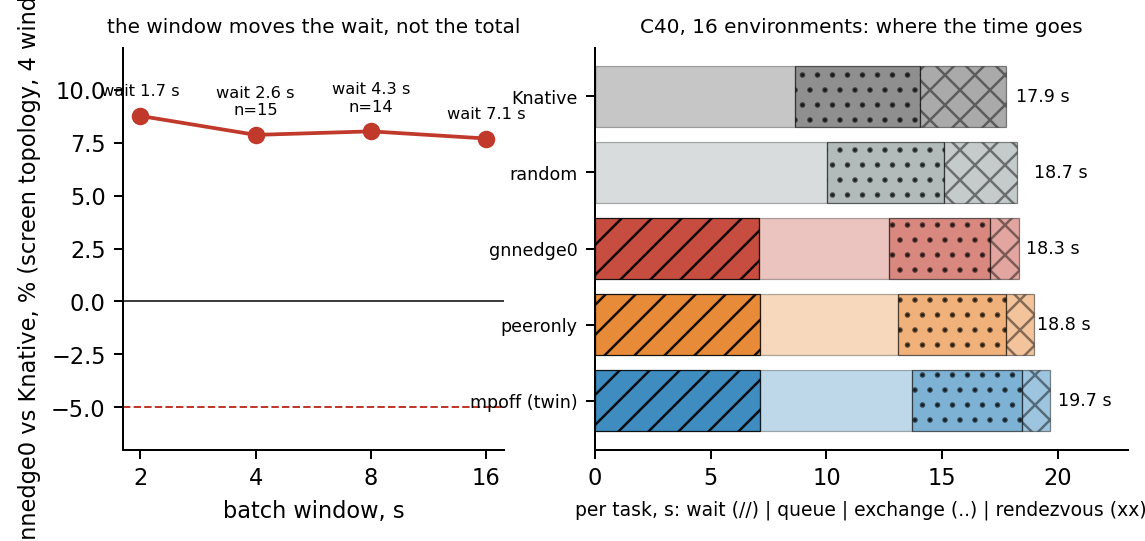
\includegraphics[width=\linewidth]{fig11_batch_window}
\caption{Left: the screen --- \code{gnnedge0} vs Knative by batch window. Right: where each
arm's time goes on the 16 study environments; hatched = scheduler wait, dotted = peer exchange,
cross-hatched = rendezvous.}
\label{fig:bw}
\end{figure}

\section{Limitations and next steps}

\begin{itemize}
  \item \textbf{Checkpoints trained at 6 servers.} Every arm was trained on a 6-server corpus;
  at 80 servers it is served $9.6\times$ out of candidate support. The 80-server null closes ``the
  existing checkpoints at scale'', not ``a GNN trained at scale''.
  \item \textbf{Synthetic peer payloads} on a real trace (\S\ref{sec:peer}). The magnitude of every
  peer-related effect depends on the 200\,MB scale; the direction of the argument does not.
  \item \textbf{The starved-client spin.} 15 of 48 cells per 6-server rung hang; it is a known
  simulator defect (a postponed task retried every batch when its client's reachable servers are
  memory-full), recorded, and excluded by a rule fixed before the data. Fixing it would widen the
  admissible set, not change a number.
  \item \textbf{w0 dependence.} The headline's history is a w0 history. Tonight's runs are the
  first that can say what it is worth elsewhere.
  \item \textbf{Next.} The window is closed as a lever, and so is removing batching outright
  ($-1731\,\%$ in an earlier lineage). The one configuration this record has never served is a
  decoder that places each arrival \emph{immediately}, conditioned on the partners already
  placed --- no group wait, no relocated rendezvous --- which the prefix-conditioned decoder
  supports in form. Whether 1.05\,s of exchange per task is worth the concentration it causes is
  then a question the same apparatus answers in an afternoon. The claim this document can make
  today is the mechanism, not a margin.
\end{itemize}

\appendix
\section{Reproducibility}
\sloppy
\begin{itemize}
  \item Record: \code{LINEAGES.md} (index) $\to$ \cpath{docs/lineages/<name>.md} (one node per
  lineage, bars signed before data); \code{docs/lessons.md}; \code{docs/hard-stops.md};
  \cpath{tests/test_record_hygiene.py} (holds the record's invariants).
  \item Tonight's lineages: \cpath{docs/lineages/unsaturated_edge_v1.md} (commits \code{96f0b69},
  \code{a7d0e72}), \cpath{docs/lineages/batch_window_edge_v1.md} (\code{f6384eb});
  readers \cpath{scripts_cosim/unsaturated_edge_v1_read.py},
  \cpath{scripts_cosim/batch_window_edge_v1_read.py} with their tests; cluster scripts under
  \cpath{scripts_cosim/datalab/}.
  \item This document: \cpath{paper/professor_summary/}; every figure regenerates from
  \cpath{make_figures.py} and the summaries under \code{data/}; the statistics are computed by the
  registered readers, so the figures show exactly the numbers the record carries.
  \item Earlier chronology: \cpath{paper/herosim_findings_report.tex} (2026-09-09).
\end{itemize}

\end{document}
